\documentclass[11pt,a4paper]{article}
\usepackage[utf8]{inputenc}
\usepackage{graphicx}

\textheight=22cm
\textwidth=14.945cm
\topmargin=0.5cm
\headheight=0cm
\headsep=0cm
\oddsidemargin=0.5cm
\evensidemargin=0.5cm
\columnsep=0.8cm
\renewcommand{\baselinestretch}{1.3}

\begin{document}

\begin{titlepage}
  \begin{center} \sloppy
    \large \textsc{Project YaJTris - Yet another Java Tetris clone }
    \vfill

    \huge \textbf{Design document} \vfill 

    \LARGE Jussi Mäki - joamaki@gmail.com
    \vspace{3mm}
    
    A programming project\\
    for Mika Holmström, University of Helsinki, Computer Science department

    \vfill

    Helsinki \today
    % \number\day .\number\month .\number\year

  \end{center}
\end{titlepage}

\section {Introduction}

This document documents the object-oriented design of YaJTris.

\section {The classes}

YaJTris is divided in to 4 classes. 

The Game class drives the game, processing keyboard input from the user, 
calling the other classes to draw objects on screen and timing and keeping track of the current game state.

The Board class is used to draw squares, clear lines and check for collisions. The Game class uses it for the actual
playing board as well for previewing the next tetromino.

The Tetromino class presents the tetris piece controlled by the user. It uses the Board class to draw the squares and 
check for collisions when moving or rotating the object. When tetromino cannot move it's information (the squares) are transferred to squares on board.

The HighScores class handels handling and drawing of the high score database.

\vspace{3mm}
\begin{center}
  %\include{class_diagram}
  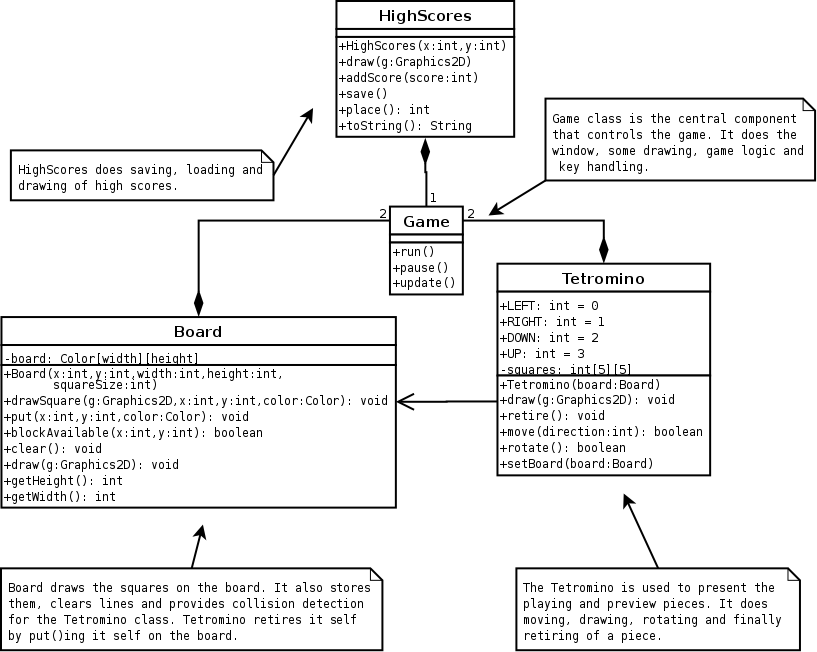
\includegraphics[scale=0.4]{class_diagram.png}
\end{center}

\newpage

\section {Class interactions}

\begin{itemize}
  \item Game logic
    \begin{center}
      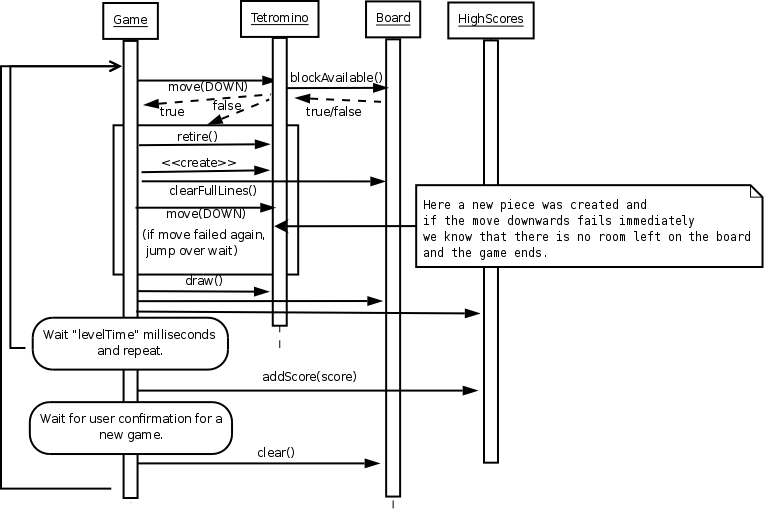
\includegraphics[scale=0.30]{seq_game.png}
    \end{center}    

  \item Rotating and moving a tetromino
    \begin{center}
      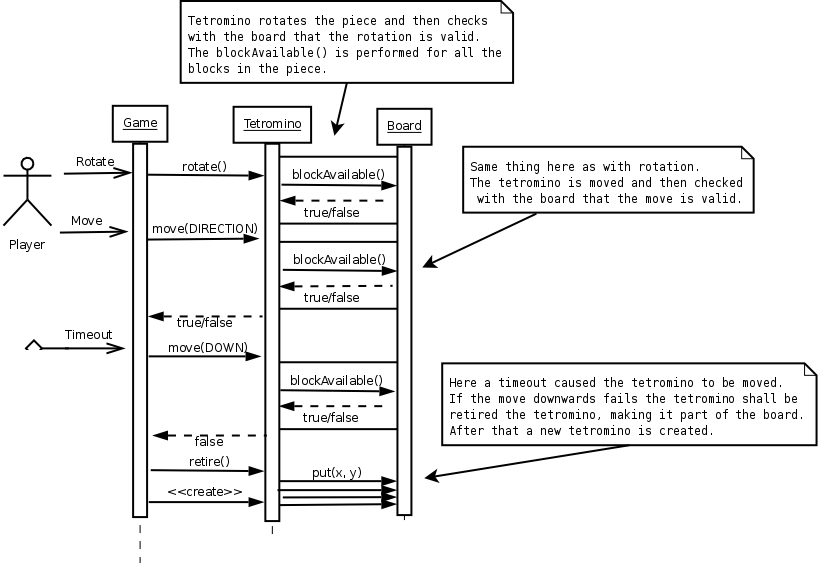
\includegraphics[scale=0.35]{seq_tetro.png}
    \end{center}
\end{itemize}

\section {User interface}

The user interface uses only a minimum amount of Java Swing components. The JPanel is used as a drawing canvas
on which the squares and scores are drawn. The program makes use of the Java2D graphics API for drawing
text and rectangles. The interface has a close resemblence to that of the original Tetris. The
Tetromino class only draws indirectly through the Board class.

The elements map to classes as follows: 
\begin{itemize}
  \item Game class draws current level and score, ie. gameInfo.
  \item The two Board class instances draw playing board on left and preview board on right.
  \item Tetromino class draws (through Board class method) the tetromino within the the two boards.
  \item HighScores class draws the high scores.
\end{itemize}

\vspace{3mm}
The element layout looks like this:
\begin{center}
  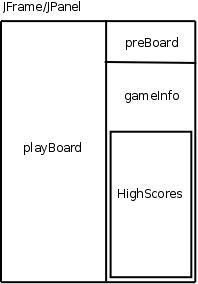
\includegraphics[scale=0.5]{uielements.png}
\end{center}

\end{document}